% Created by tikzDevice version 0.12.6 on 2026-08-10 06:16:18
% !TEX encoding = UTF-8 Unicode
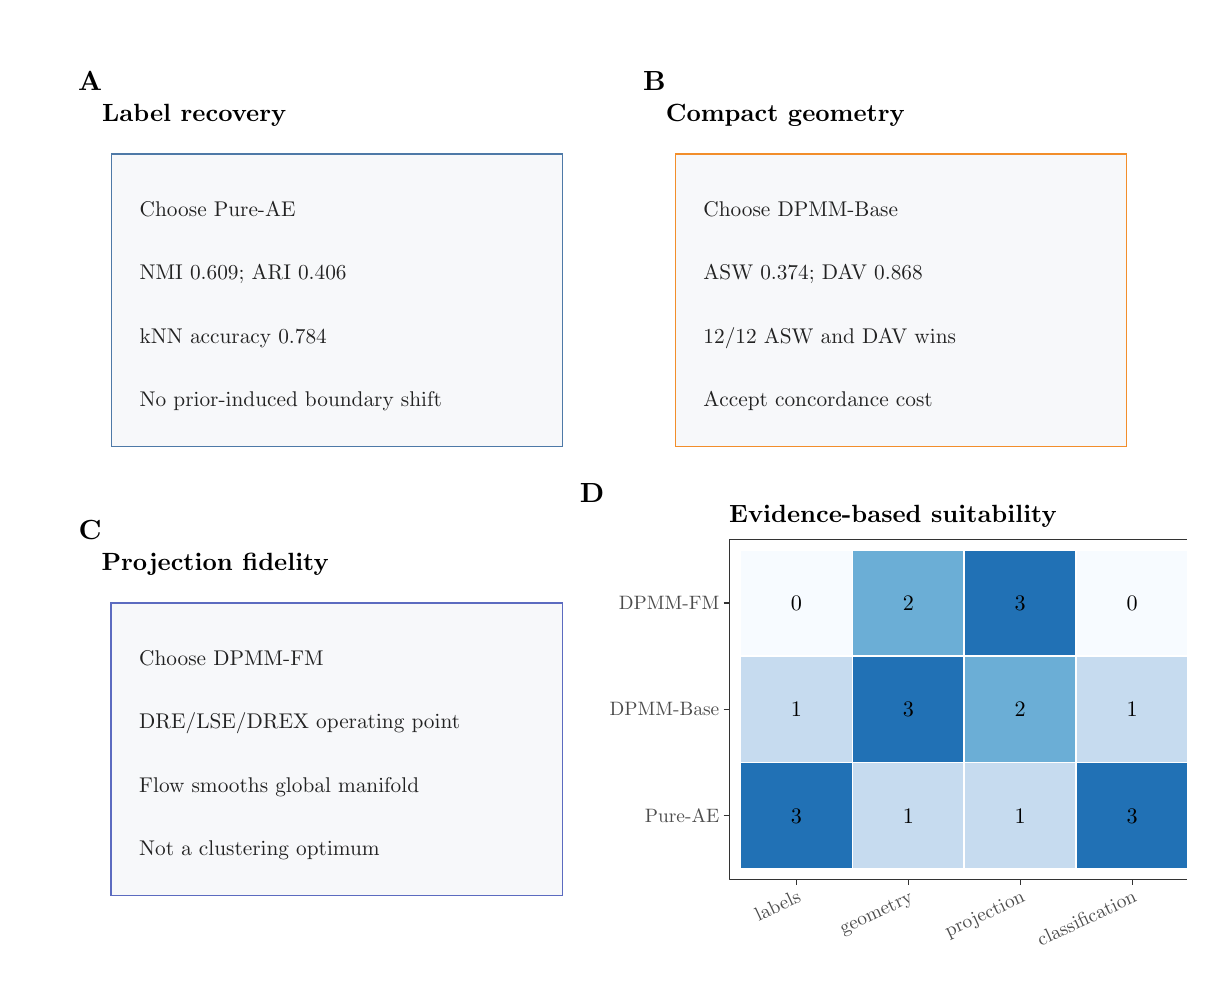
\begin{tikzpicture}[x=1pt,y=1pt]
\definecolor{fillColor}{RGB}{255,255,255}
\path[use as bounding box,fill=fillColor,fill opacity=0.00] (0,0) rectangle (418.91,335.46);
\begin{scope}
\path[clip] (  0.00,  0.00) rectangle (418.91,335.46);
\definecolor{drawColor}{RGB}{255,255,255}
\definecolor{fillColor}{RGB}{255,255,255}

\path[draw=drawColor,line width= 0.6pt,line join=round,line cap=round,fill=fillColor] (  0.00,  0.00) rectangle (418.91,335.46);
\end{scope}
\begin{scope}
\path[clip] (  5.50,167.73) rectangle (209.45,329.96);
\definecolor{drawColor}{RGB}{255,255,255}
\definecolor{fillColor}{RGB}{255,255,255}

\path[draw=drawColor,line width= 0.6pt,line join=round,line cap=round,fill=fillColor] (  5.50,167.73) rectangle (209.45,329.96);
\end{scope}
\begin{scope}
\path[clip] (209.45,167.73) rectangle (413.41,329.96);
\definecolor{drawColor}{RGB}{255,255,255}
\definecolor{fillColor}{RGB}{255,255,255}

\path[draw=drawColor,line width= 0.6pt,line join=round,line cap=round,fill=fillColor] (209.45,167.73) rectangle (413.41,329.96);
\end{scope}
\begin{scope}
\path[clip] ( 16.21,174.76) rectangle (198.74,322.93);

\path[] ( 16.21,174.76) rectangle (198.74,322.93);
\end{scope}
\begin{scope}
\path[clip] ( 26.91,176.76) rectangle (196.74,299.62);
\definecolor{drawColor}{RGB}{78,121,167}
\definecolor{fillColor}{RGB}{247,248,250}

\path[draw=drawColor,line width= 0.5pt,fill=fillColor] ( 30.30,184.14) rectangle (193.34,289.79);
\definecolor{drawColor}{RGB}{34,34,34}

\node[text=drawColor,anchor=base west,inner sep=0pt, outer sep=0pt, scale=  0.77] at ( 40.49,267.30) {Choose Pure-AE};

\node[text=drawColor,anchor=base west,inner sep=0pt, outer sep=0pt, scale=  0.77] at ( 40.49,244.37) {NMI 0.609; ARI 0.406};

\node[text=drawColor,anchor=base west,inner sep=0pt, outer sep=0pt, scale=  0.77] at ( 40.49,221.44) {kNN accuracy 0.784};

\node[text=drawColor,anchor=base west,inner sep=0pt, outer sep=0pt, scale=  0.77] at ( 40.49,198.50) {No prior-induced boundary shift};
\end{scope}
\begin{scope}
\path[clip] (  0.00,  0.00) rectangle (418.91,335.46);
\definecolor{drawColor}{RGB}{0,0,0}

\node[text=drawColor,anchor=base west,inner sep=0pt, outer sep=0pt, scale=  0.90] at ( 26.91,301.61) {\bfseries Label recovery};
\end{scope}
\begin{scope}
\path[clip] (  0.00,  0.00) rectangle (418.91,335.46);
\definecolor{drawColor}{RGB}{0,0,0}

\node[text=drawColor,anchor=base,inner sep=0pt, outer sep=0pt, scale=  1.00] at ( 22.56,312.93) {\bfseries A};
\end{scope}
\begin{scope}
\path[clip] (220.42,174.76) rectangle (402.44,322.93);

\path[] (220.42,174.76) rectangle (402.44,322.93);
\end{scope}
\begin{scope}
\path[clip] (230.60,176.76) rectangle (400.44,299.62);
\definecolor{drawColor}{RGB}{242,142,43}
\definecolor{fillColor}{RGB}{247,248,250}

\path[draw=drawColor,line width= 0.5pt,fill=fillColor] (234.00,184.14) rectangle (397.04,289.79);
\definecolor{drawColor}{RGB}{34,34,34}

\node[text=drawColor,anchor=base west,inner sep=0pt, outer sep=0pt, scale=  0.77] at (244.19,267.30) {Choose DPMM-Base};

\node[text=drawColor,anchor=base west,inner sep=0pt, outer sep=0pt, scale=  0.77] at (244.19,244.37) {ASW 0.374; DAV 0.868};

\node[text=drawColor,anchor=base west,inner sep=0pt, outer sep=0pt, scale=  0.77] at (244.19,221.44) {12/12 ASW and DAV wins};

\node[text=drawColor,anchor=base west,inner sep=0pt, outer sep=0pt, scale=  0.77] at (244.19,198.50) {Accept concordance cost};
\end{scope}
\begin{scope}
\path[clip] (  0.00,  0.00) rectangle (418.91,335.46);
\definecolor{drawColor}{RGB}{0,0,0}

\node[text=drawColor,anchor=base west,inner sep=0pt, outer sep=0pt, scale=  0.90] at (230.60,301.61) {\bfseries Compact geometry};
\end{scope}
\begin{scope}
\path[clip] (  0.00,  0.00) rectangle (418.91,335.46);
\definecolor{drawColor}{RGB}{0,0,0}

\node[text=drawColor,anchor=base,inner sep=0pt, outer sep=0pt, scale=  1.00] at (226.51,312.93) {\bfseries B};
\end{scope}
\begin{scope}
\path[clip] (  5.50,  5.50) rectangle (209.45,167.73);
\definecolor{drawColor}{RGB}{255,255,255}
\definecolor{fillColor}{RGB}{255,255,255}

\path[draw=drawColor,line width= 0.6pt,line join=round,line cap=round,fill=fillColor] (  5.50,  5.50) rectangle (209.45,167.73);
\end{scope}
\begin{scope}
\path[clip] (209.45,  5.50) rectangle (413.41,167.73);
\definecolor{drawColor}{RGB}{255,255,255}
\definecolor{fillColor}{RGB}{255,255,255}

\path[draw=drawColor,line width= 0.6pt,line join=round,line cap=round,fill=fillColor] (209.45,  5.50) rectangle (413.41,167.73);
\end{scope}
\begin{scope}
\path[clip] ( 16.41, 12.53) rectangle (198.55,160.70);

\path[] ( 16.41, 12.53) rectangle (198.55,160.70);
\end{scope}
\begin{scope}
\path[clip] ( 26.71, 14.53) rectangle (196.55,137.39);
\definecolor{drawColor}{RGB}{92,107,192}
\definecolor{fillColor}{RGB}{247,248,250}

\path[draw=drawColor,line width= 0.5pt,fill=fillColor] ( 30.11, 21.90) rectangle (193.15,127.56);
\definecolor{drawColor}{RGB}{34,34,34}

\node[text=drawColor,anchor=base west,inner sep=0pt, outer sep=0pt, scale=  0.77] at ( 40.30,105.07) {Choose DPMM-FM};

\node[text=drawColor,anchor=base west,inner sep=0pt, outer sep=0pt, scale=  0.77] at ( 40.30, 82.14) {DRE/LSE/DREX operating point};

\node[text=drawColor,anchor=base west,inner sep=0pt, outer sep=0pt, scale=  0.77] at ( 40.30, 59.20) {Flow smooths global manifold};

\node[text=drawColor,anchor=base west,inner sep=0pt, outer sep=0pt, scale=  0.77] at ( 40.30, 36.27) {Not a clustering optimum};
\end{scope}
\begin{scope}
\path[clip] (  0.00,  0.00) rectangle (418.91,335.46);
\definecolor{drawColor}{RGB}{0,0,0}

\node[text=drawColor,anchor=base west,inner sep=0pt, outer sep=0pt, scale=  0.90] at ( 26.71,139.38) {\bfseries Projection fidelity};
\end{scope}
\begin{scope}
\path[clip] (  0.00,  0.00) rectangle (418.91,335.46);
\definecolor{drawColor}{RGB}{0,0,0}

\node[text=drawColor,anchor=base,inner sep=0pt, outer sep=0pt, scale=  1.00] at ( 22.56,150.69) {\bfseries C};
\end{scope}
\begin{scope}
\path[clip] (197.51,  0.00) rectangle (418.91,173.90);
\definecolor{drawColor}{RGB}{255,255,255}
\definecolor{fillColor}{RGB}{255,255,255}

\path[draw=drawColor,line width= 0.4pt,line join=round,line cap=round,fill=fillColor] (197.51, -0.67) rectangle (425.35,173.90);
\end{scope}
\begin{scope}
\path[clip] (253.51, 27.73) rectangle (418.91,150.59);
\definecolor{fillColor}{RGB}{255,255,255}

\path[fill=fillColor] (253.51, 27.73) rectangle (423.35,150.59);
\definecolor{drawColor}{RGB}{255,255,255}
\definecolor{fillColor}{RGB}{33,113,181}

\path[draw=drawColor,line width= 0.6pt,fill=fillColor] (257.56, 31.57) rectangle (297.99, 69.97);
\definecolor{fillColor}{RGB}{198,219,239}

\path[draw=drawColor,line width= 0.6pt,fill=fillColor] (257.56, 69.97) rectangle (297.99,108.36);
\definecolor{fillColor}{RGB}{247,251,255}

\path[draw=drawColor,line width= 0.6pt,fill=fillColor] (257.56,108.36) rectangle (297.99,146.75);
\definecolor{fillColor}{RGB}{198,219,239}

\path[draw=drawColor,line width= 0.6pt,fill=fillColor] (297.99, 31.57) rectangle (338.43, 69.97);
\definecolor{fillColor}{RGB}{33,113,181}

\path[draw=drawColor,line width= 0.6pt,fill=fillColor] (297.99, 69.97) rectangle (338.43,108.36);
\definecolor{fillColor}{RGB}{107,174,214}

\path[draw=drawColor,line width= 0.6pt,fill=fillColor] (297.99,108.36) rectangle (338.43,146.75);
\definecolor{fillColor}{RGB}{198,219,239}

\path[draw=drawColor,line width= 0.6pt,fill=fillColor] (338.43, 31.57) rectangle (378.87, 69.97);
\definecolor{fillColor}{RGB}{107,174,214}

\path[draw=drawColor,line width= 0.6pt,fill=fillColor] (338.43, 69.97) rectangle (378.87,108.36);
\definecolor{fillColor}{RGB}{33,113,181}

\path[draw=drawColor,line width= 0.6pt,fill=fillColor] (338.43,108.36) rectangle (378.87,146.75);

\path[draw=drawColor,line width= 0.6pt,fill=fillColor] (378.87, 31.57) rectangle (419.30, 69.97);
\definecolor{fillColor}{RGB}{198,219,239}

\path[draw=drawColor,line width= 0.6pt,fill=fillColor] (378.87, 69.97) rectangle (419.30,108.36);
\definecolor{fillColor}{RGB}{247,251,255}

\path[draw=drawColor,line width= 0.6pt,fill=fillColor] (378.87,108.36) rectangle (419.30,146.75);
\definecolor{drawColor}{RGB}{0,0,0}

\node[text=drawColor,anchor=base,inner sep=0pt, outer sep=0pt, scale=  0.80] at (277.77, 48.03) {3};

\node[text=drawColor,anchor=base,inner sep=0pt, outer sep=0pt, scale=  0.80] at (277.77, 86.42) {1};

\node[text=drawColor,anchor=base,inner sep=0pt, outer sep=0pt, scale=  0.80] at (277.77,124.81) {0};

\node[text=drawColor,anchor=base,inner sep=0pt, outer sep=0pt, scale=  0.80] at (318.21, 48.03) {1};

\node[text=drawColor,anchor=base,inner sep=0pt, outer sep=0pt, scale=  0.80] at (318.21, 86.42) {3};

\node[text=drawColor,anchor=base,inner sep=0pt, outer sep=0pt, scale=  0.80] at (318.21,124.81) {2};

\node[text=drawColor,anchor=base,inner sep=0pt, outer sep=0pt, scale=  0.80] at (358.65, 48.03) {1};

\node[text=drawColor,anchor=base,inner sep=0pt, outer sep=0pt, scale=  0.80] at (358.65, 86.42) {2};

\node[text=drawColor,anchor=base,inner sep=0pt, outer sep=0pt, scale=  0.80] at (358.65,124.81) {3};

\node[text=drawColor,anchor=base,inner sep=0pt, outer sep=0pt, scale=  0.80] at (399.09, 48.03) {3};

\node[text=drawColor,anchor=base,inner sep=0pt, outer sep=0pt, scale=  0.80] at (399.09, 86.42) {1};

\node[text=drawColor,anchor=base,inner sep=0pt, outer sep=0pt, scale=  0.80] at (399.09,124.81) {0};
\definecolor{drawColor}{gray}{0.20}

\path[draw=drawColor,line width= 0.4pt,line join=round,line cap=round] (253.51, 27.73) rectangle (423.35,150.59);
\end{scope}
\begin{scope}
\path[clip] (  0.00,  0.00) rectangle (418.91,335.46);
\definecolor{drawColor}{gray}{0.30}

\node[text=drawColor,anchor=base east,inner sep=0pt, outer sep=0pt, scale=  0.70] at (249.91, 48.36) {Pure-AE};

\node[text=drawColor,anchor=base east,inner sep=0pt, outer sep=0pt, scale=  0.70] at (249.91, 86.75) {DPMM-Base};

\node[text=drawColor,anchor=base east,inner sep=0pt, outer sep=0pt, scale=  0.70] at (249.91,125.15) {DPMM-FM};
\end{scope}
\begin{scope}
\path[clip] (  0.00,  0.00) rectangle (418.91,335.46);
\definecolor{drawColor}{gray}{0.20}

\path[draw=drawColor,line width= 0.4pt,line join=round] (251.51, 50.77) --
	(253.51, 50.77);

\path[draw=drawColor,line width= 0.4pt,line join=round] (251.51, 89.16) --
	(253.51, 89.16);

\path[draw=drawColor,line width= 0.4pt,line join=round] (251.51,127.56) --
	(253.51,127.56);
\end{scope}
\begin{scope}
\path[clip] (  0.00,  0.00) rectangle (418.91,335.46);
\definecolor{drawColor}{gray}{0.20}

\path[draw=drawColor,line width= 0.4pt,line join=round] (277.77, 25.73) --
	(277.77, 27.73);

\path[draw=drawColor,line width= 0.4pt,line join=round] (318.21, 25.73) --
	(318.21, 27.73);

\path[draw=drawColor,line width= 0.4pt,line join=round] (358.65, 25.73) --
	(358.65, 27.73);

\path[draw=drawColor,line width= 0.4pt,line join=round] (399.09, 25.73) --
	(399.09, 27.73);
\end{scope}
\begin{scope}
\path[clip] (  0.00,  0.00) rectangle (418.91,335.46);
\definecolor{drawColor}{gray}{0.30}

\node[text=drawColor,rotate= 25.00,anchor=base east,inner sep=0pt, outer sep=0pt, scale=  0.70] at (279.81, 19.76) {labels};

\node[text=drawColor,rotate= 25.00,anchor=base east,inner sep=0pt, outer sep=0pt, scale=  0.70] at (320.25, 19.76) {geometry};

\node[text=drawColor,rotate= 25.00,anchor=base east,inner sep=0pt, outer sep=0pt, scale=  0.70] at (360.69, 19.76) {projection};

\node[text=drawColor,rotate= 25.00,anchor=base east,inner sep=0pt, outer sep=0pt, scale=  0.70] at (401.12, 19.76) {classification};
\end{scope}
\begin{scope}
\path[clip] (  0.00,  0.00) rectangle (418.91,335.46);
\definecolor{drawColor}{RGB}{0,0,0}

\node[text=drawColor,anchor=base west,inner sep=0pt, outer sep=0pt, scale=  0.90] at (253.51,156.58) {\bfseries Evidence-based suitability};
\end{scope}
\begin{scope}
\path[clip] (  0.00,  0.00) rectangle (418.91,335.46);
\definecolor{drawColor}{RGB}{0,0,0}

\node[text=drawColor,anchor=base,inner sep=0pt, outer sep=0pt, scale=  1.00] at (203.92,163.90) {\bfseries D};
\end{scope}
\end{tikzpicture}
